\section{Procedure}
\subsection{Bridge}
Overview of the bridge’s procedure
\setenumerate[2]{label=\arabic*.}
\begin{enumerate}
\item Producing basic paper beams 
\item Producing bridge’s main long beams
\item Producing paper stripes
\item Assembling one side of the bridge
\item Connecting two sides of the bridge to form the structure
\end{enumerate}

\begin{enumerate}
\item Producing basic paper beams
\item Producing bridge’s main long beams
	\begin{enumerate}
	\item Measure 3 cm from the right side of a beam.
	\item Place the forepart of the scissors into the hollow area of the beam. Cut off the right side of the beam by 3 cm along only one of its diagonals.
	(picture)
	\item Apply glue on the inner surface of the cut beam from the right side of the beam by 3 cm.
	\item Plug the left side of another beam into the right side of the former beam straightly. 
	\textbf{Caution:} be careful with the direction of two beams, and they should be a straight line. 
	\item Repeat step1 to step 4 on the second, the third, the fourth and the fifth beams. 
	\item Use electric hair drier to dry the connection part of the long beam, which is composed by 5 basic paper beams. 
	\item Use pencil to mart the middle of the long beam. Measure 25 cm, 50 cm, and 53 cm from the middle point to both sides of the beam. Mark these four points on the beam respectively. 
	\item Repeat step1 to 7 to produce another long beam. 
	\end{enumerate}
\item Producing paper stripes
	\begin{enumerate}
	\item Cut a script of 0.5 cm $\times$ 29.7 cm paper scripts from A4 papers by an art knife. 
	\item Repeat step 1 to produce 16 scripts of scripts.
	\item Apply glue to connect 2 stripes. The connection part of the scripts should be 1 cm. Produce 4 middle stripes in this way.
	\item Apply glue to connect 4 stripes one by one. The connection part of the scripts should be 1 cm. Produce 2 long strips in this way.
	\item Use electric hair drier to dry the connection part of stripes.
	\end{enumerate}
\item Assembling one side of the bridge
	\begin{enumerate}
	\item Use an art knife to incise a 6 cm $\times$ 0.5 cm $\times$ 1 cm short pillow from basic beams. Produce 2 short pillow in this way. 
	\item Place the forepart of the scissors into the hollow area of the pillow. Cut off the right side of the beam by 1 cm along both of its diagonals.
	(picture)
	\item Turn out four pieces of the cut pillow, and apply glue on each of the four pieces respectively. 
	\item Paste four pieces to the bottom of the main long beam on the mark of 25 cm, wrapping the beam. In this way, paste 2 short pillows to the 25 cm marks on both sides of the long beam. 
	Caution: the center line of the pillow should fit the mark.
	\item Use an art knife to incise a 11 cm $\times$ 0.5 cm $\times$ 1 cm short pillow from basic beams. Produce 1 short pillow in this way. 
	\item Place the forepart of the scissors into the hollow area of the pillow. Cut off the right side of the beam by 1 cm along both of its diagonals.
	(picture)
	\item Turn out four pieces of the cut pillow, and apply glue on each of the four pieces respectively. 
	\item Paste four pieces to the bottom of the main long beam on the mark of the middle point, wrapping the beam. 
	Caution: the center line of the pillow should fit the mark.
	\item Use electric hair drier to dry the connection part. 
	\item Cut three pieces of 2.5 cm $\times$ 1 cm paper stripes. Paste them on the other side of three pillows, covering their hollow areas respectively.
	(picture)
	\item Paste the middle stripes on the mark of 50 cm, then paste it on the top of the short pillow, and paste it by the bottom side of the long pillow. Paste the remaining part of the script along the beam and the side surface of the long pillow respectively. Paste two middle stripes on both sides of the main beam respectively. 
	(picture)
	\item Paste the long stripe on the mark of 50 cm, then paste it on the top of the long pillow, and paste it on the other side’s 50 cm mark of the main beam.
	(picture)
	\item Cut three pieces of 3.5 cm $\times$ 2 cm paper. Wrap the connection part above with a piece of paper respectively. 
	\item Use electric hair drier to dry the connection part.
	\end{enumerate}
\item Connecting two sides of the bridge to form the structure
	\begin{enumerate}
	\item Use an art knife to incise a 16.4 cm $\times$ 0.5 cm $\times$ 1 cm beam from basic beams. Produce 2 beams in this way. Incise a 4 cm $\times$ 0.5 cm $\times$ 1 cm beam from basic beams. Produce 4 beams in this way.
	\item Place the forepart of the scissors into the hollow area of beams. Cut off the both sides of the 16.4 cm $\times$ 0.5 cm $\times$ 1 cm beam by 1 cm along both of its diagonals. Cut off the both sides of the 4 cm $\times$ 0.5 cm $\times$ 1 cm beam by 1 cm along both of its diagonals.
	\item Turn out 8 pieces of the cut beam, and apply glue on each of these pieces respectively. 
	\item Paste the 16.4 cm $\times$ 0.5 cm $\times$ 1 cm beam on the 136.5 cm  $\times$ 1 cm inner plane of the beam just by the 50 cm mark. Use turned pieces to wrap the main beam. Do the same thing on the other side of the beam with the other side’s bridge.
	(picture) 
	\item Repeat step 3 and step 4 to connect another side of the whole bridge.
	\item Turn out 4 pieces of the cut beam, and apply glue on each of these pieces respectively. 
	\item Paste the 4 cm $\times$ 0.5 cm $\times$ 1 cm beam on the 136.5 cm  $\times$ 1 cm inside plane of the beam just by the 53 cm mark. Paste another 4 cm $\times$ 0.5 cm $\times$ 1 cm beam on the 136.5 cm  $\times$ 1 cm outside plane of the beam just beside the former beam. Use turned pieces to wrap the main beam. 
	\item Repeat step 6 and step 7 for 4 times to paste other six 4 cm $\times$ 0.5 cm $\times$ 1 cm beams to each side of each side bridge of the whole structure. 
	(picture)
	\item Use electric hair drier to dry the connection part. 
	\end{enumerate}
\end{enumerate}

\subsection{Cart}
Constructing process of cart
\begin{enumerate}
\item Constructing the base
	\begin{enumerate}
	\item	Draw an 13.0 cm $\times$ 10.0 cm baseboard on the computer software AutoCAD.\\
	\begin{figure}
	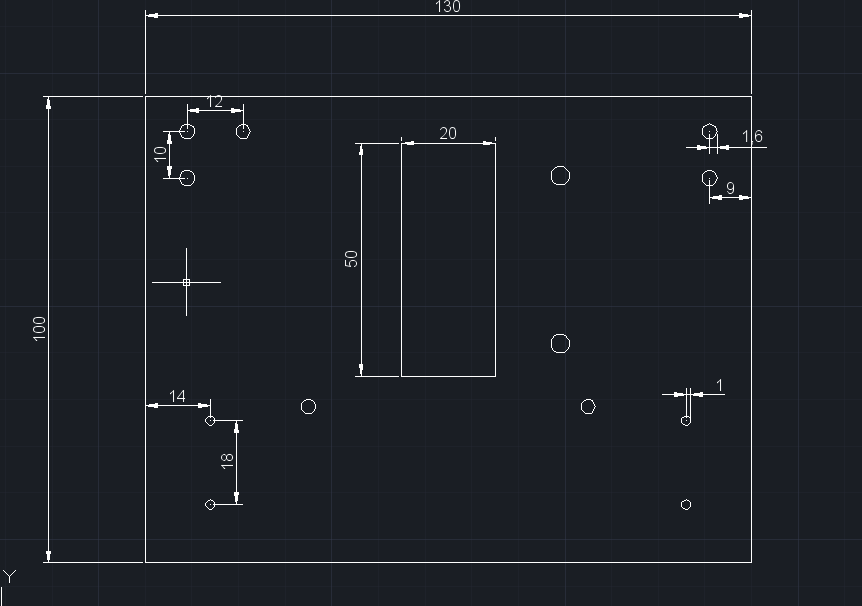
\includegraphics[height=10cm]{figure/procedure/p1}
 	\caption{CAD drawing \label{fig:cad}}
	\end{figure}
	\item Cut 2 mm-thick carbon fibre board according to the design drawing. Notice: Since only limited information can be illustrated on this figure, you can decide the distance between holes by yourself. You may go through some measurements. There are three types of holes on the board. You can identify them from the size on the figure. The product is as follow. \\
	\begin{figure}
	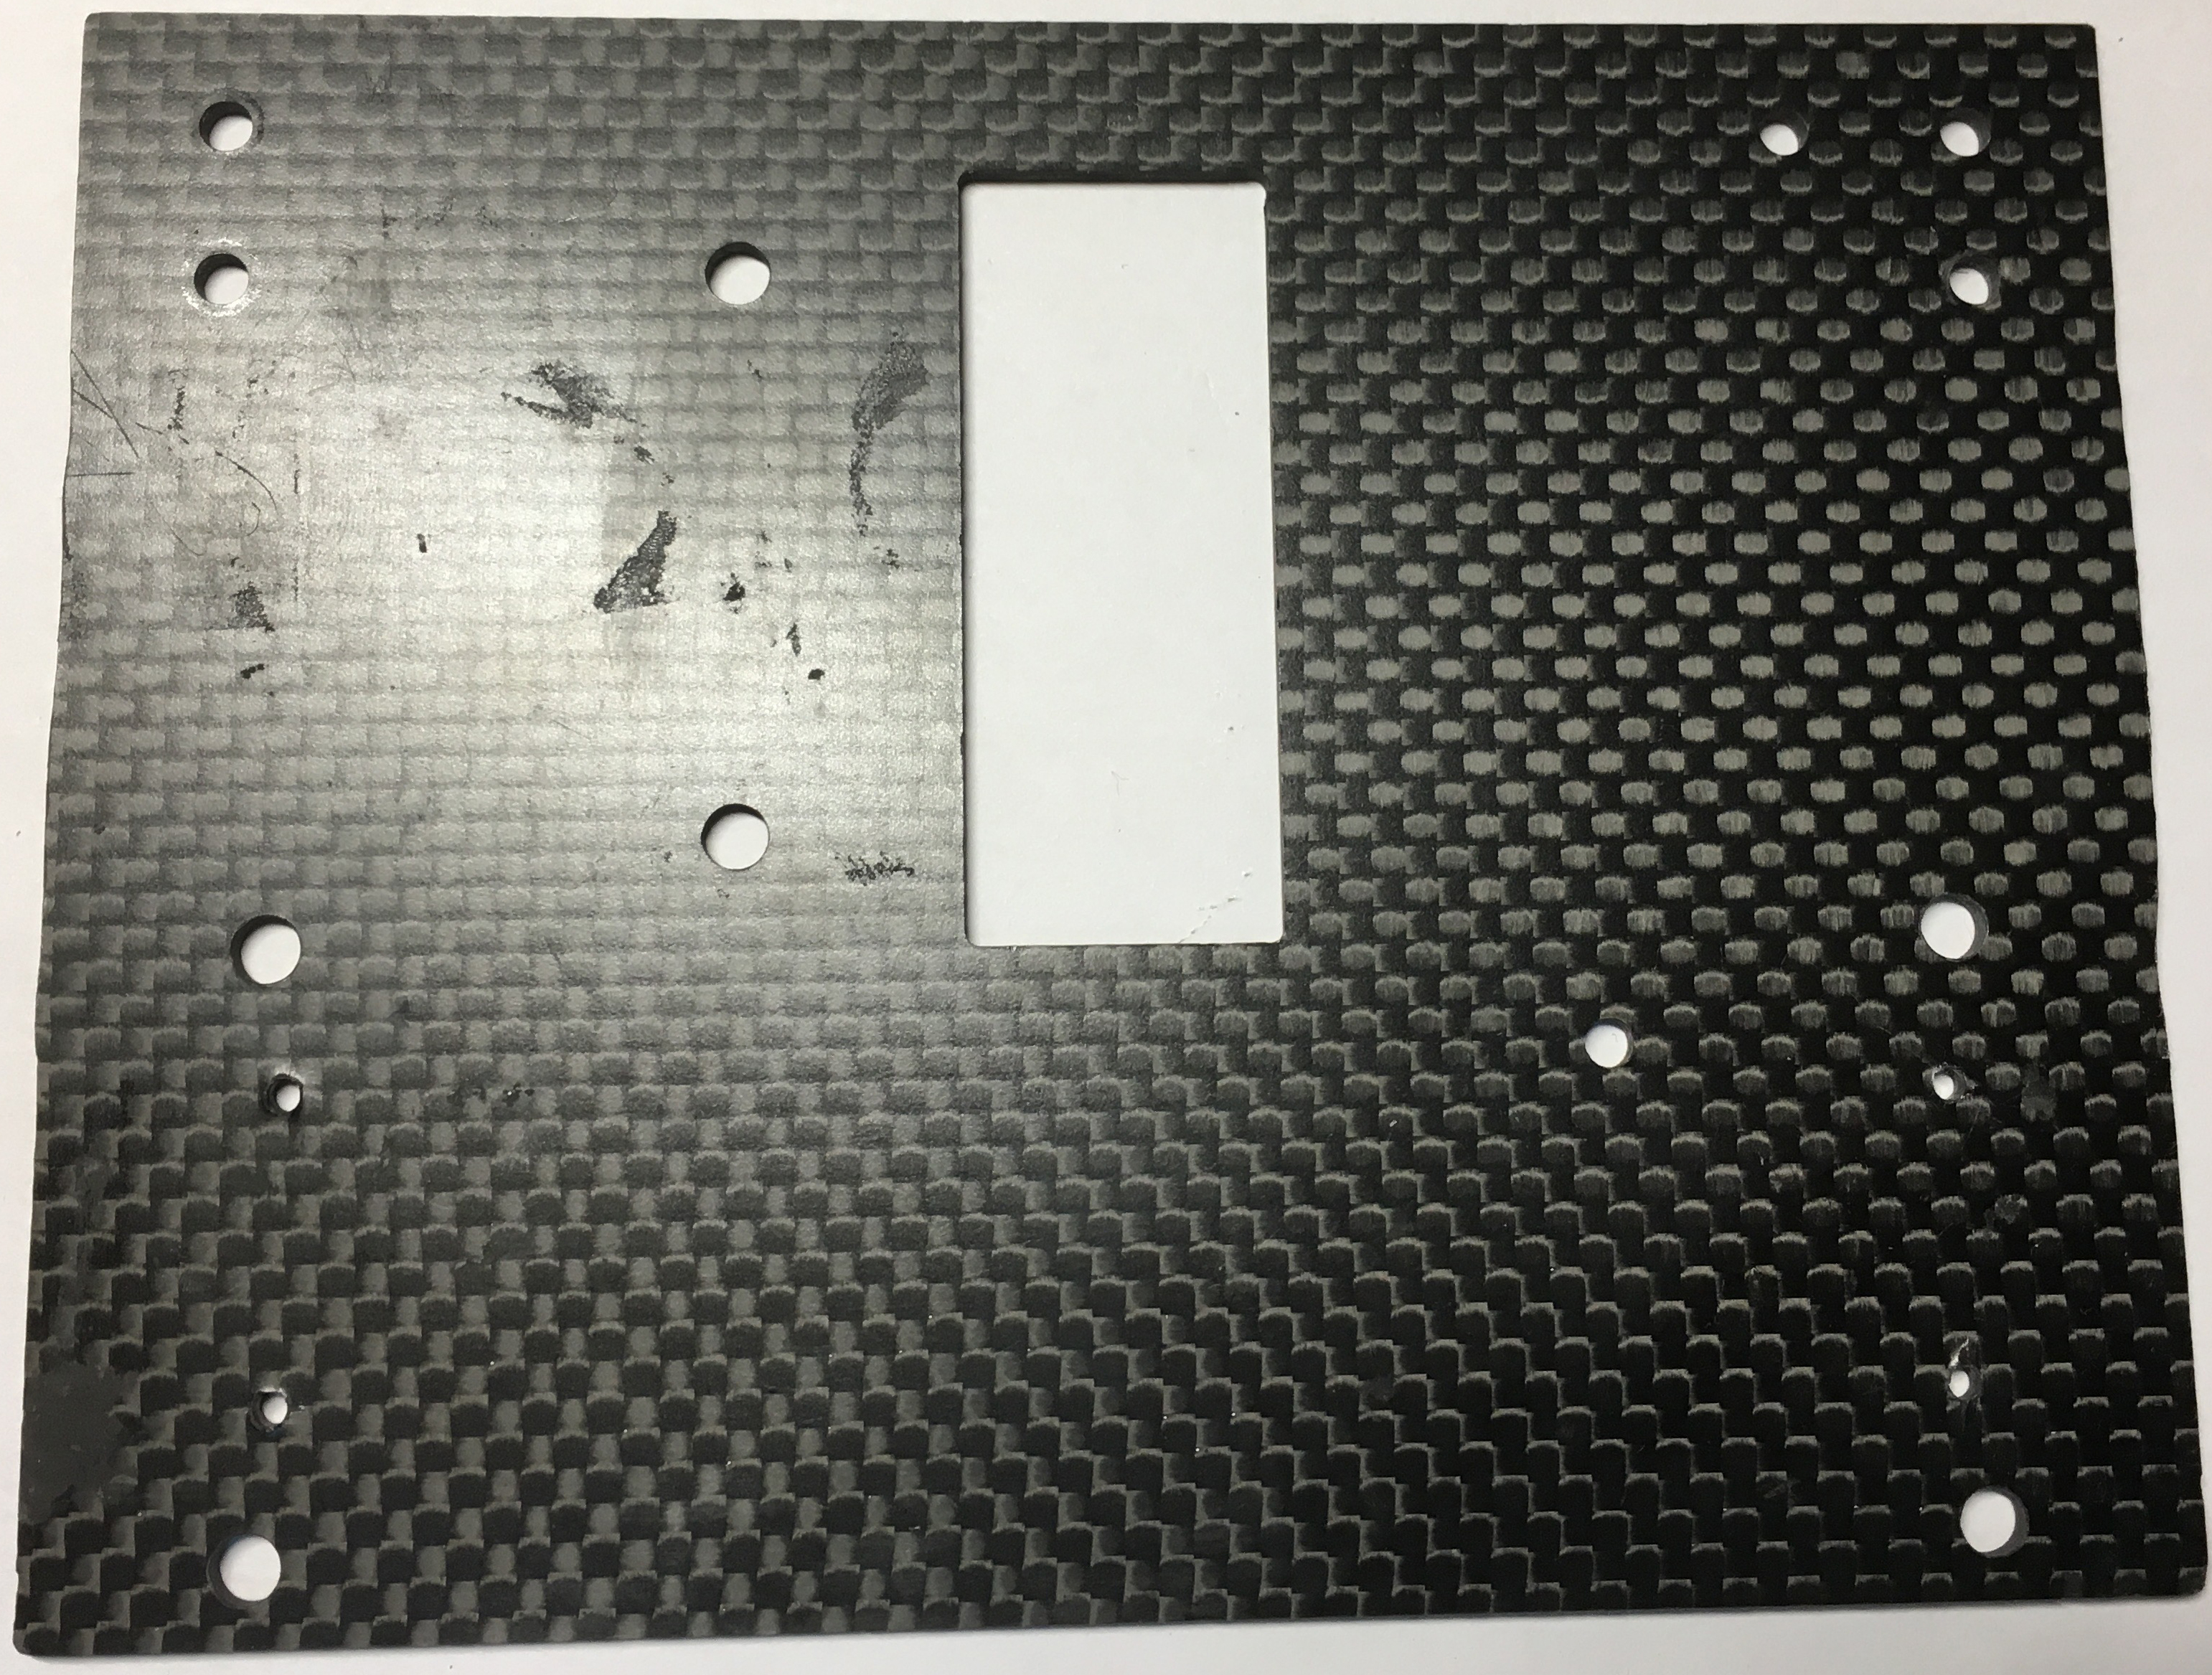
\includegraphics[height=10cm]{figure/procedure/p2}
 	\caption{Carbon fibre board \label{fig:carbonFiberBoard}}
	\end{figure}
	\end{enumerate}
\item Design circuit diagram 
\item Design wheels
	\begin{enumerate}
	\item Draw a wheel with radius of 2.3 cm on the computer software Solidworks.\\
	\begin{figure}
	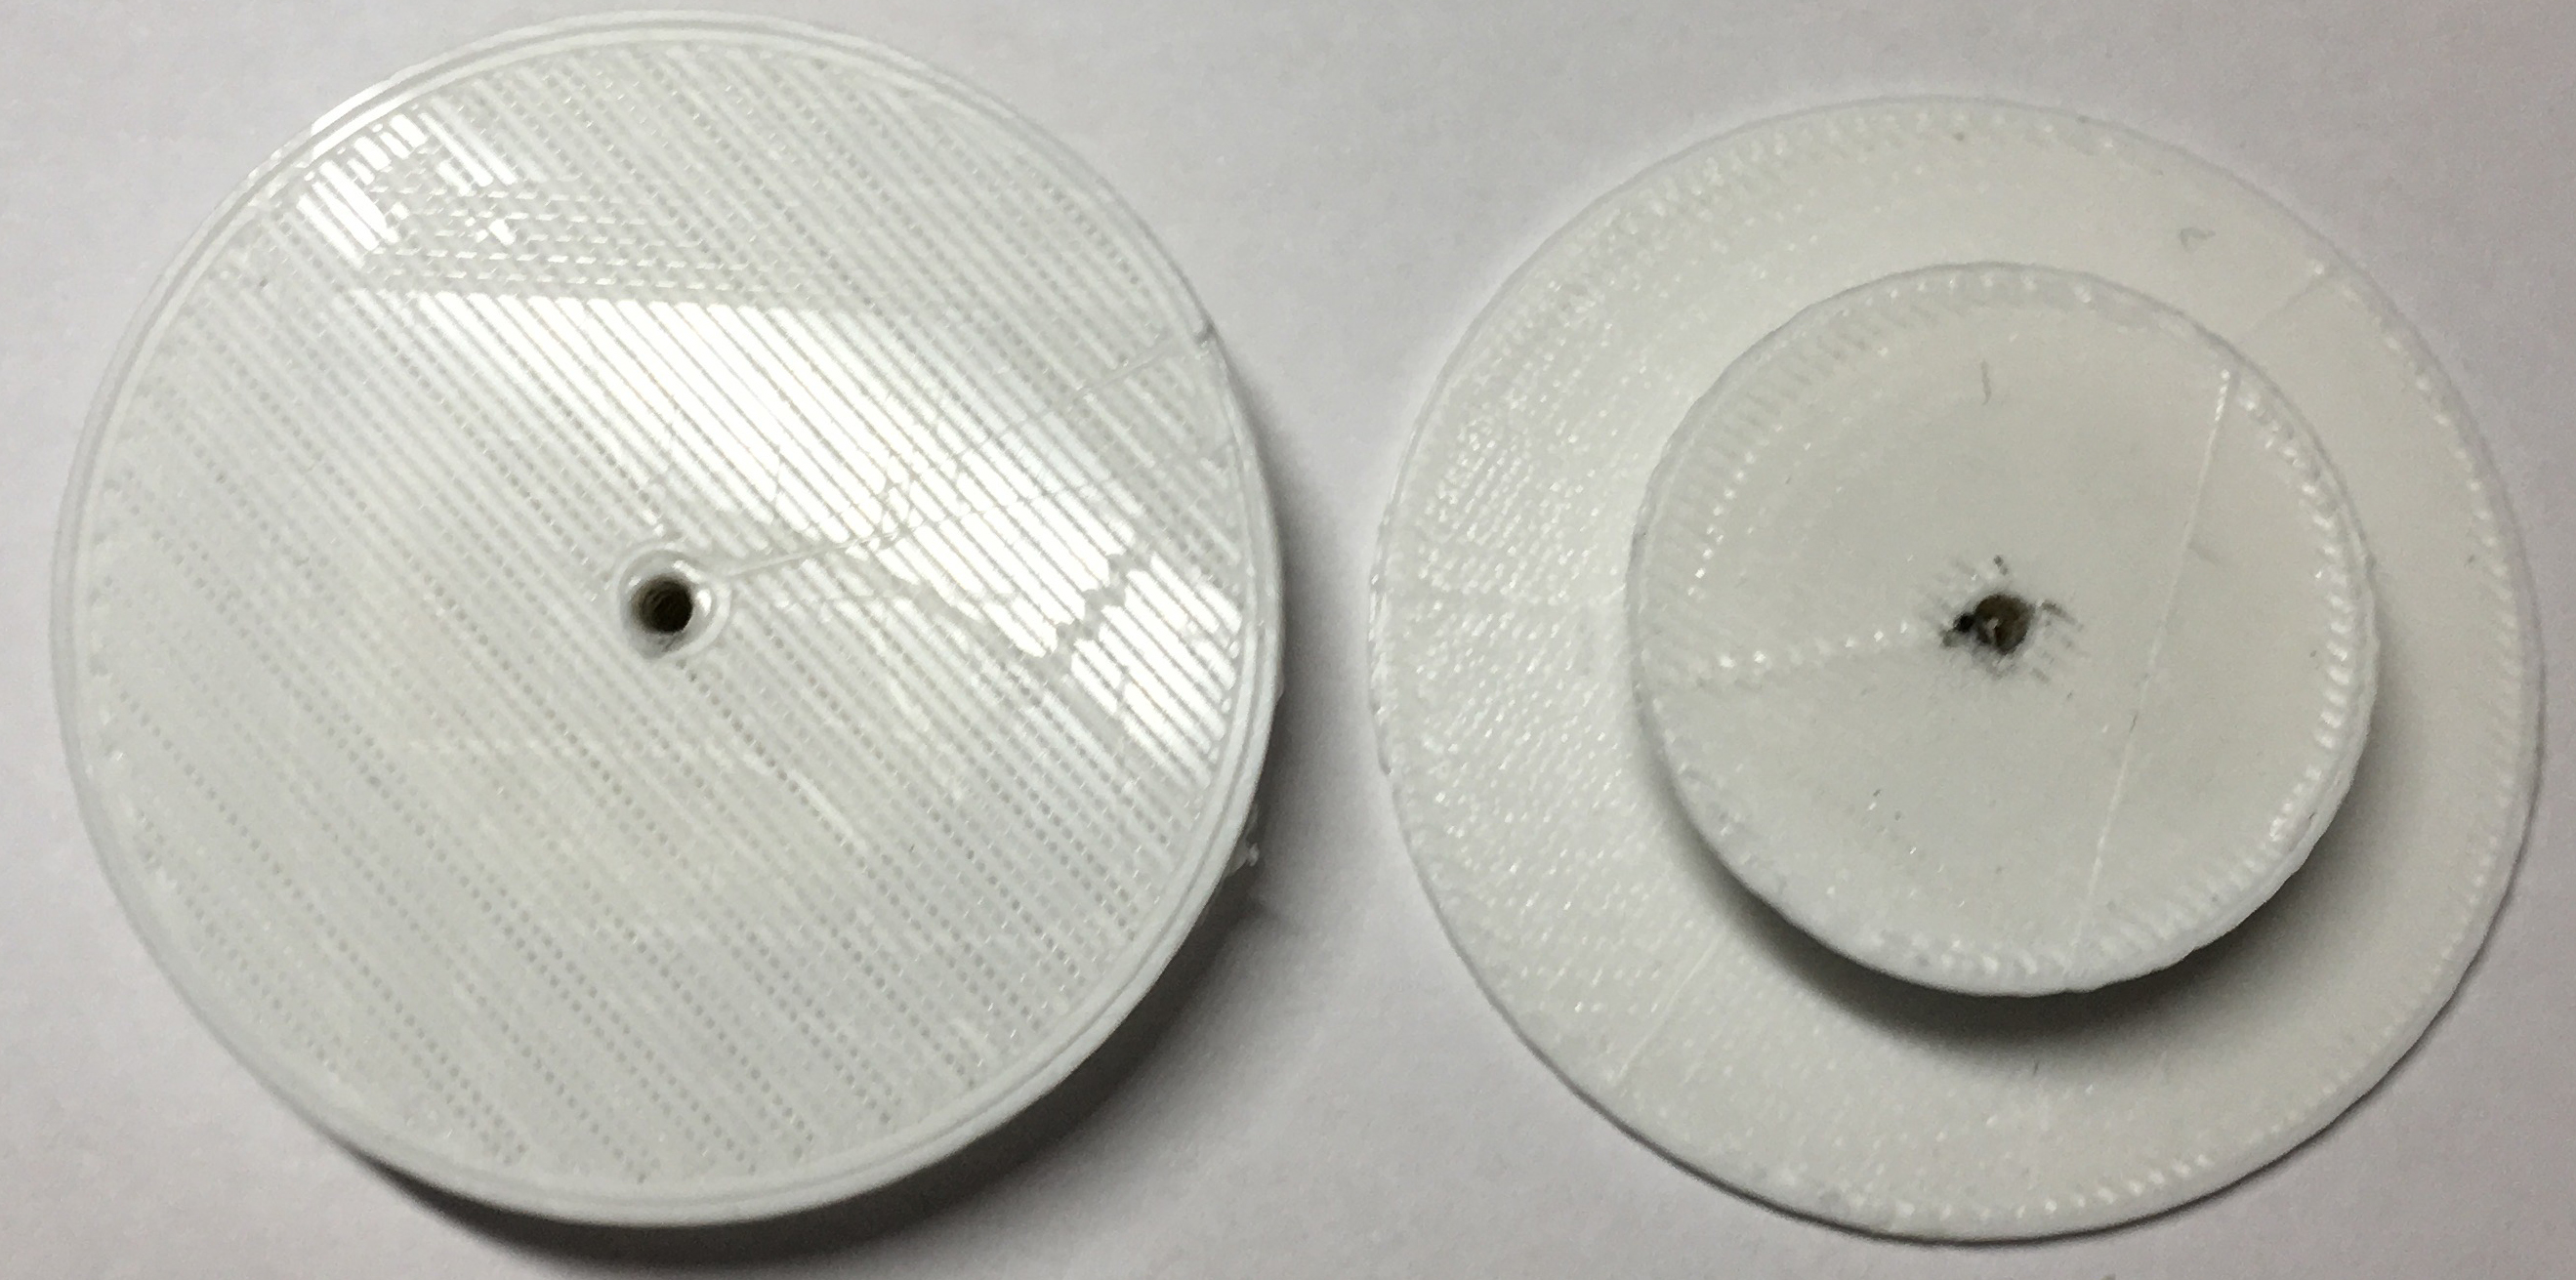
\includegraphics[height=10cm]{figure/procedure/p3}
 	\caption{Wheels \label{fig:wheels}}
	\end{figure}
	\item Print two wheels according the ``STL'' file in 3D.
	\end{enumerate}
\item Assembling Motor, Servo and Wheels
	\begin{enumerate}
	\item Fix two stators at two corners of the base from below with screws and nuts. 
	\item Fix two N20 motors and back wheels at the other two corners of the base from above with screws and nuts.
	\item Insert a carbon fibre axle in to the hole of the two stators. \textbf{Caution:} Make sure the length on two sides beyond the stators the same. \\
	\begin{figure}[H]
	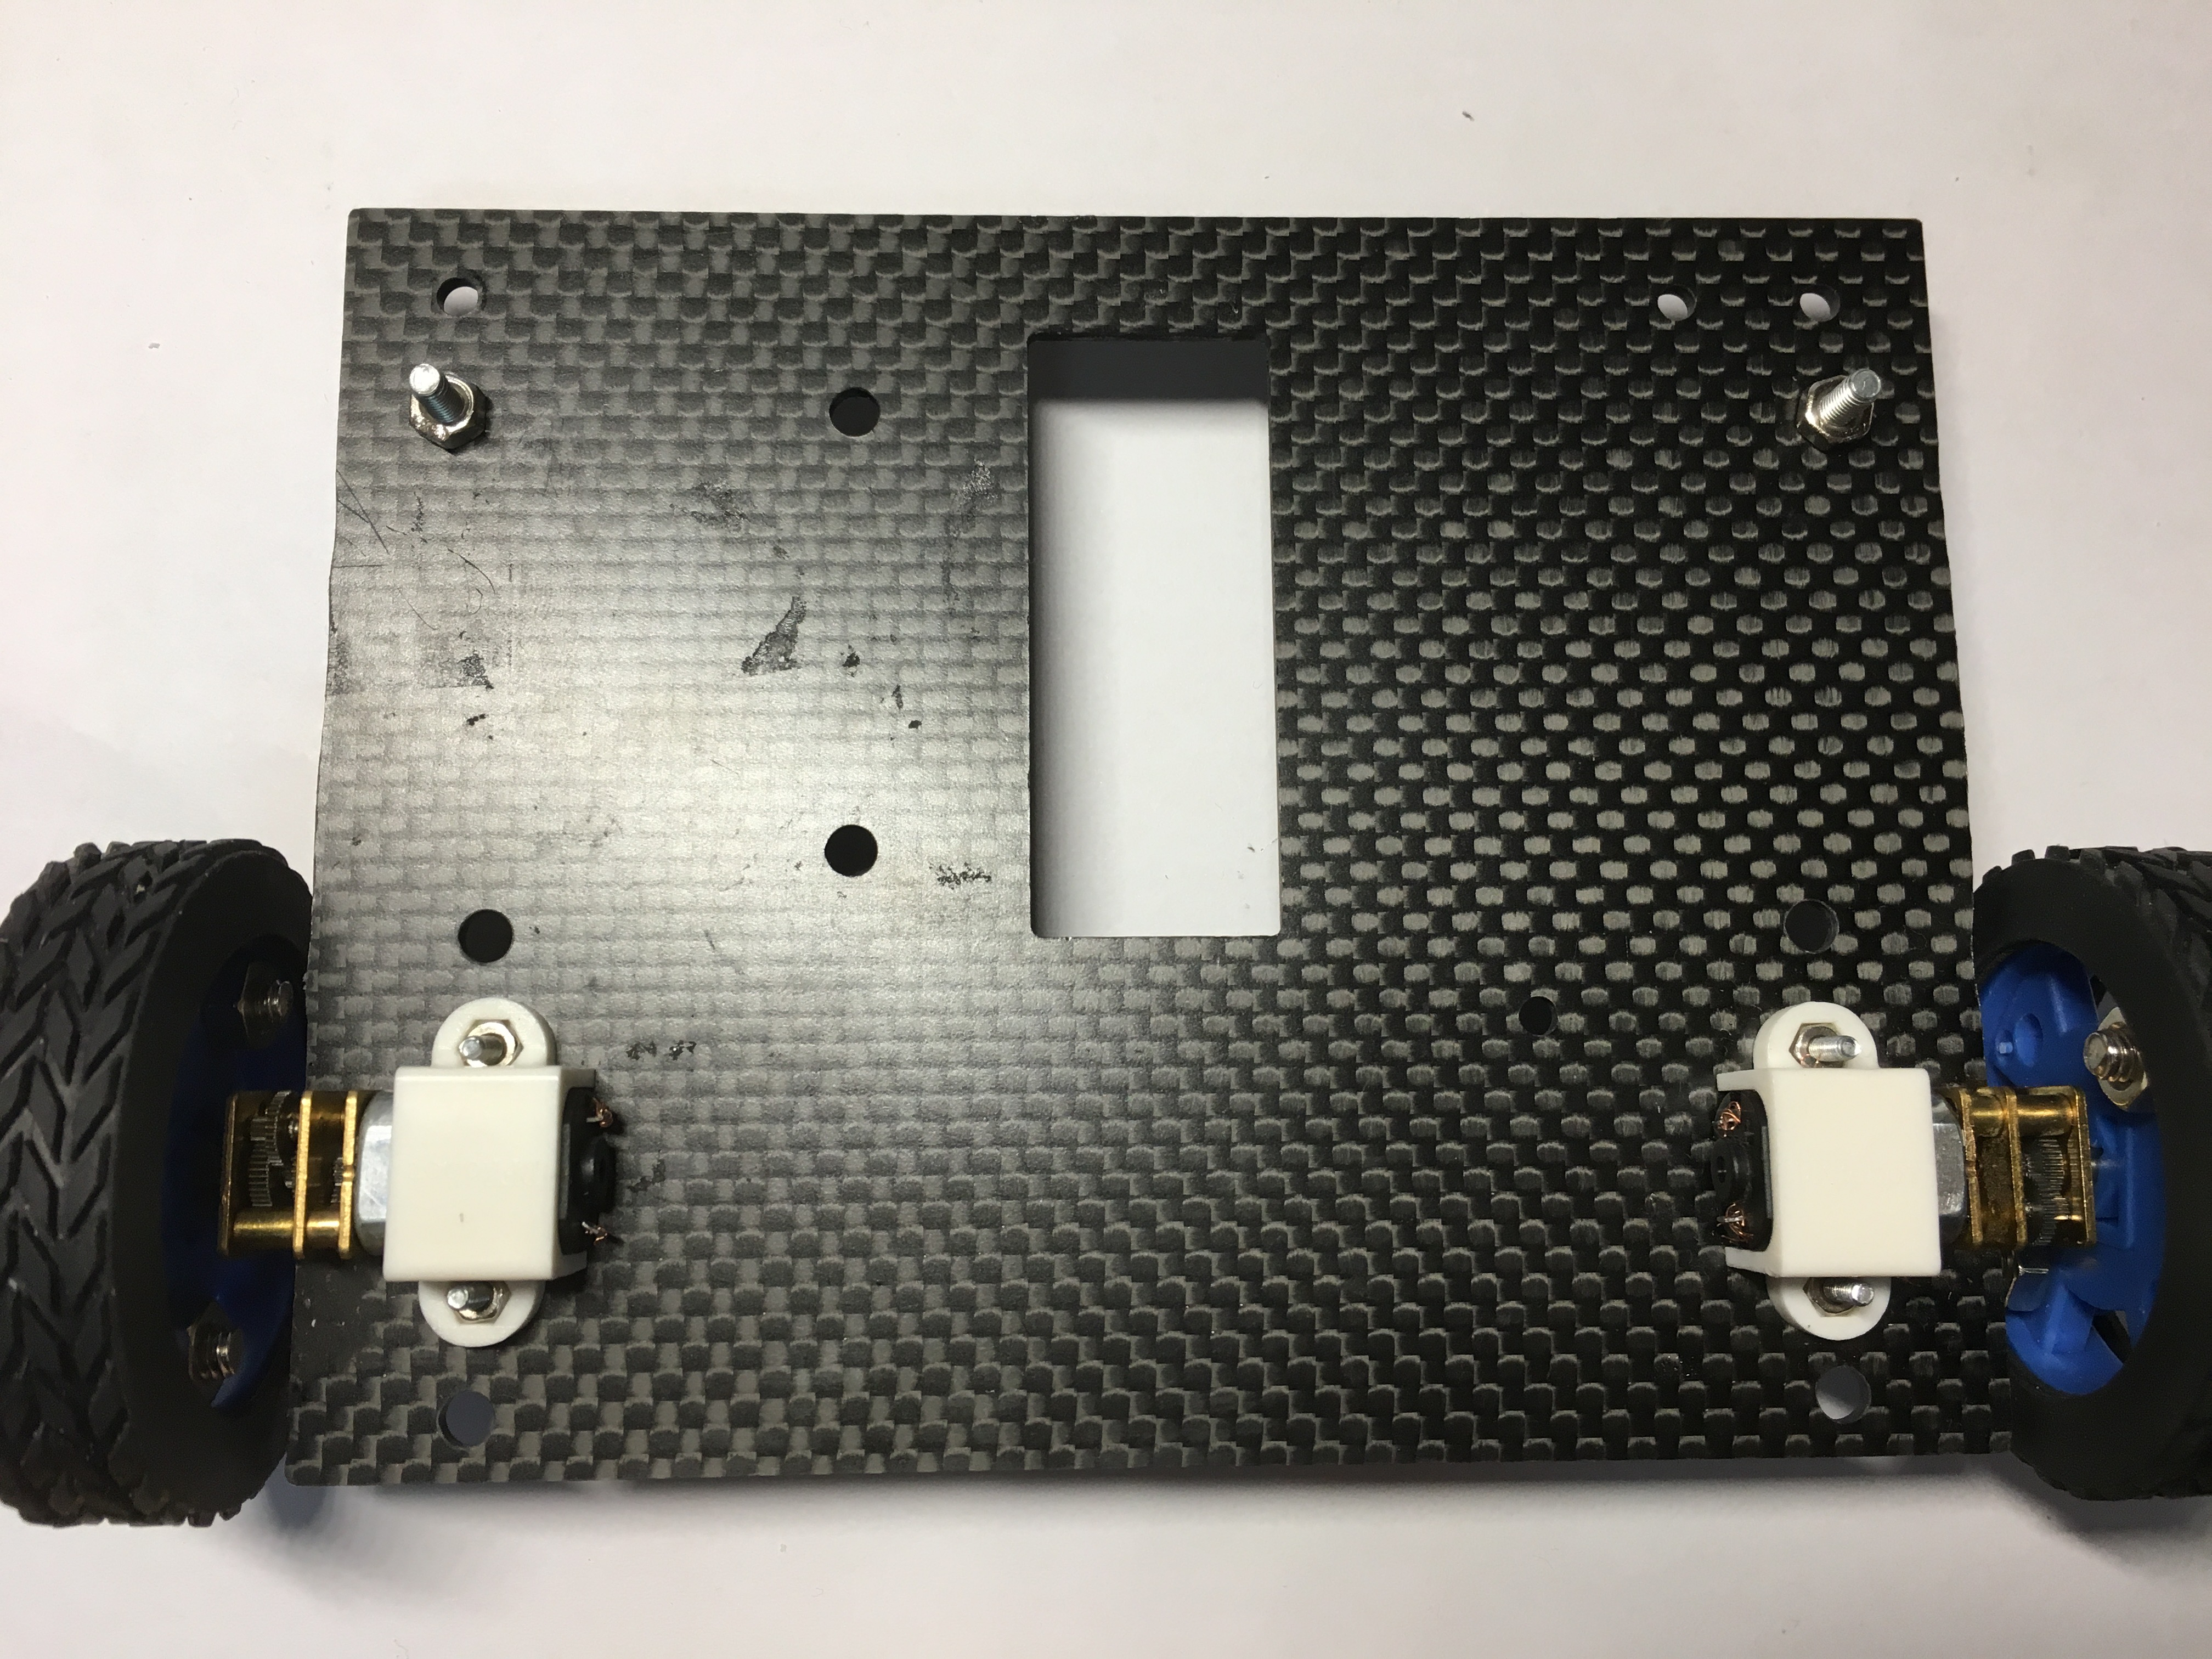
\includegraphics[height=10cm]{figure/procedure/p4}
 	\caption{Step 4.3 \label{fig:step43}}
	\end{figure}
	\begin{figure}[H]
	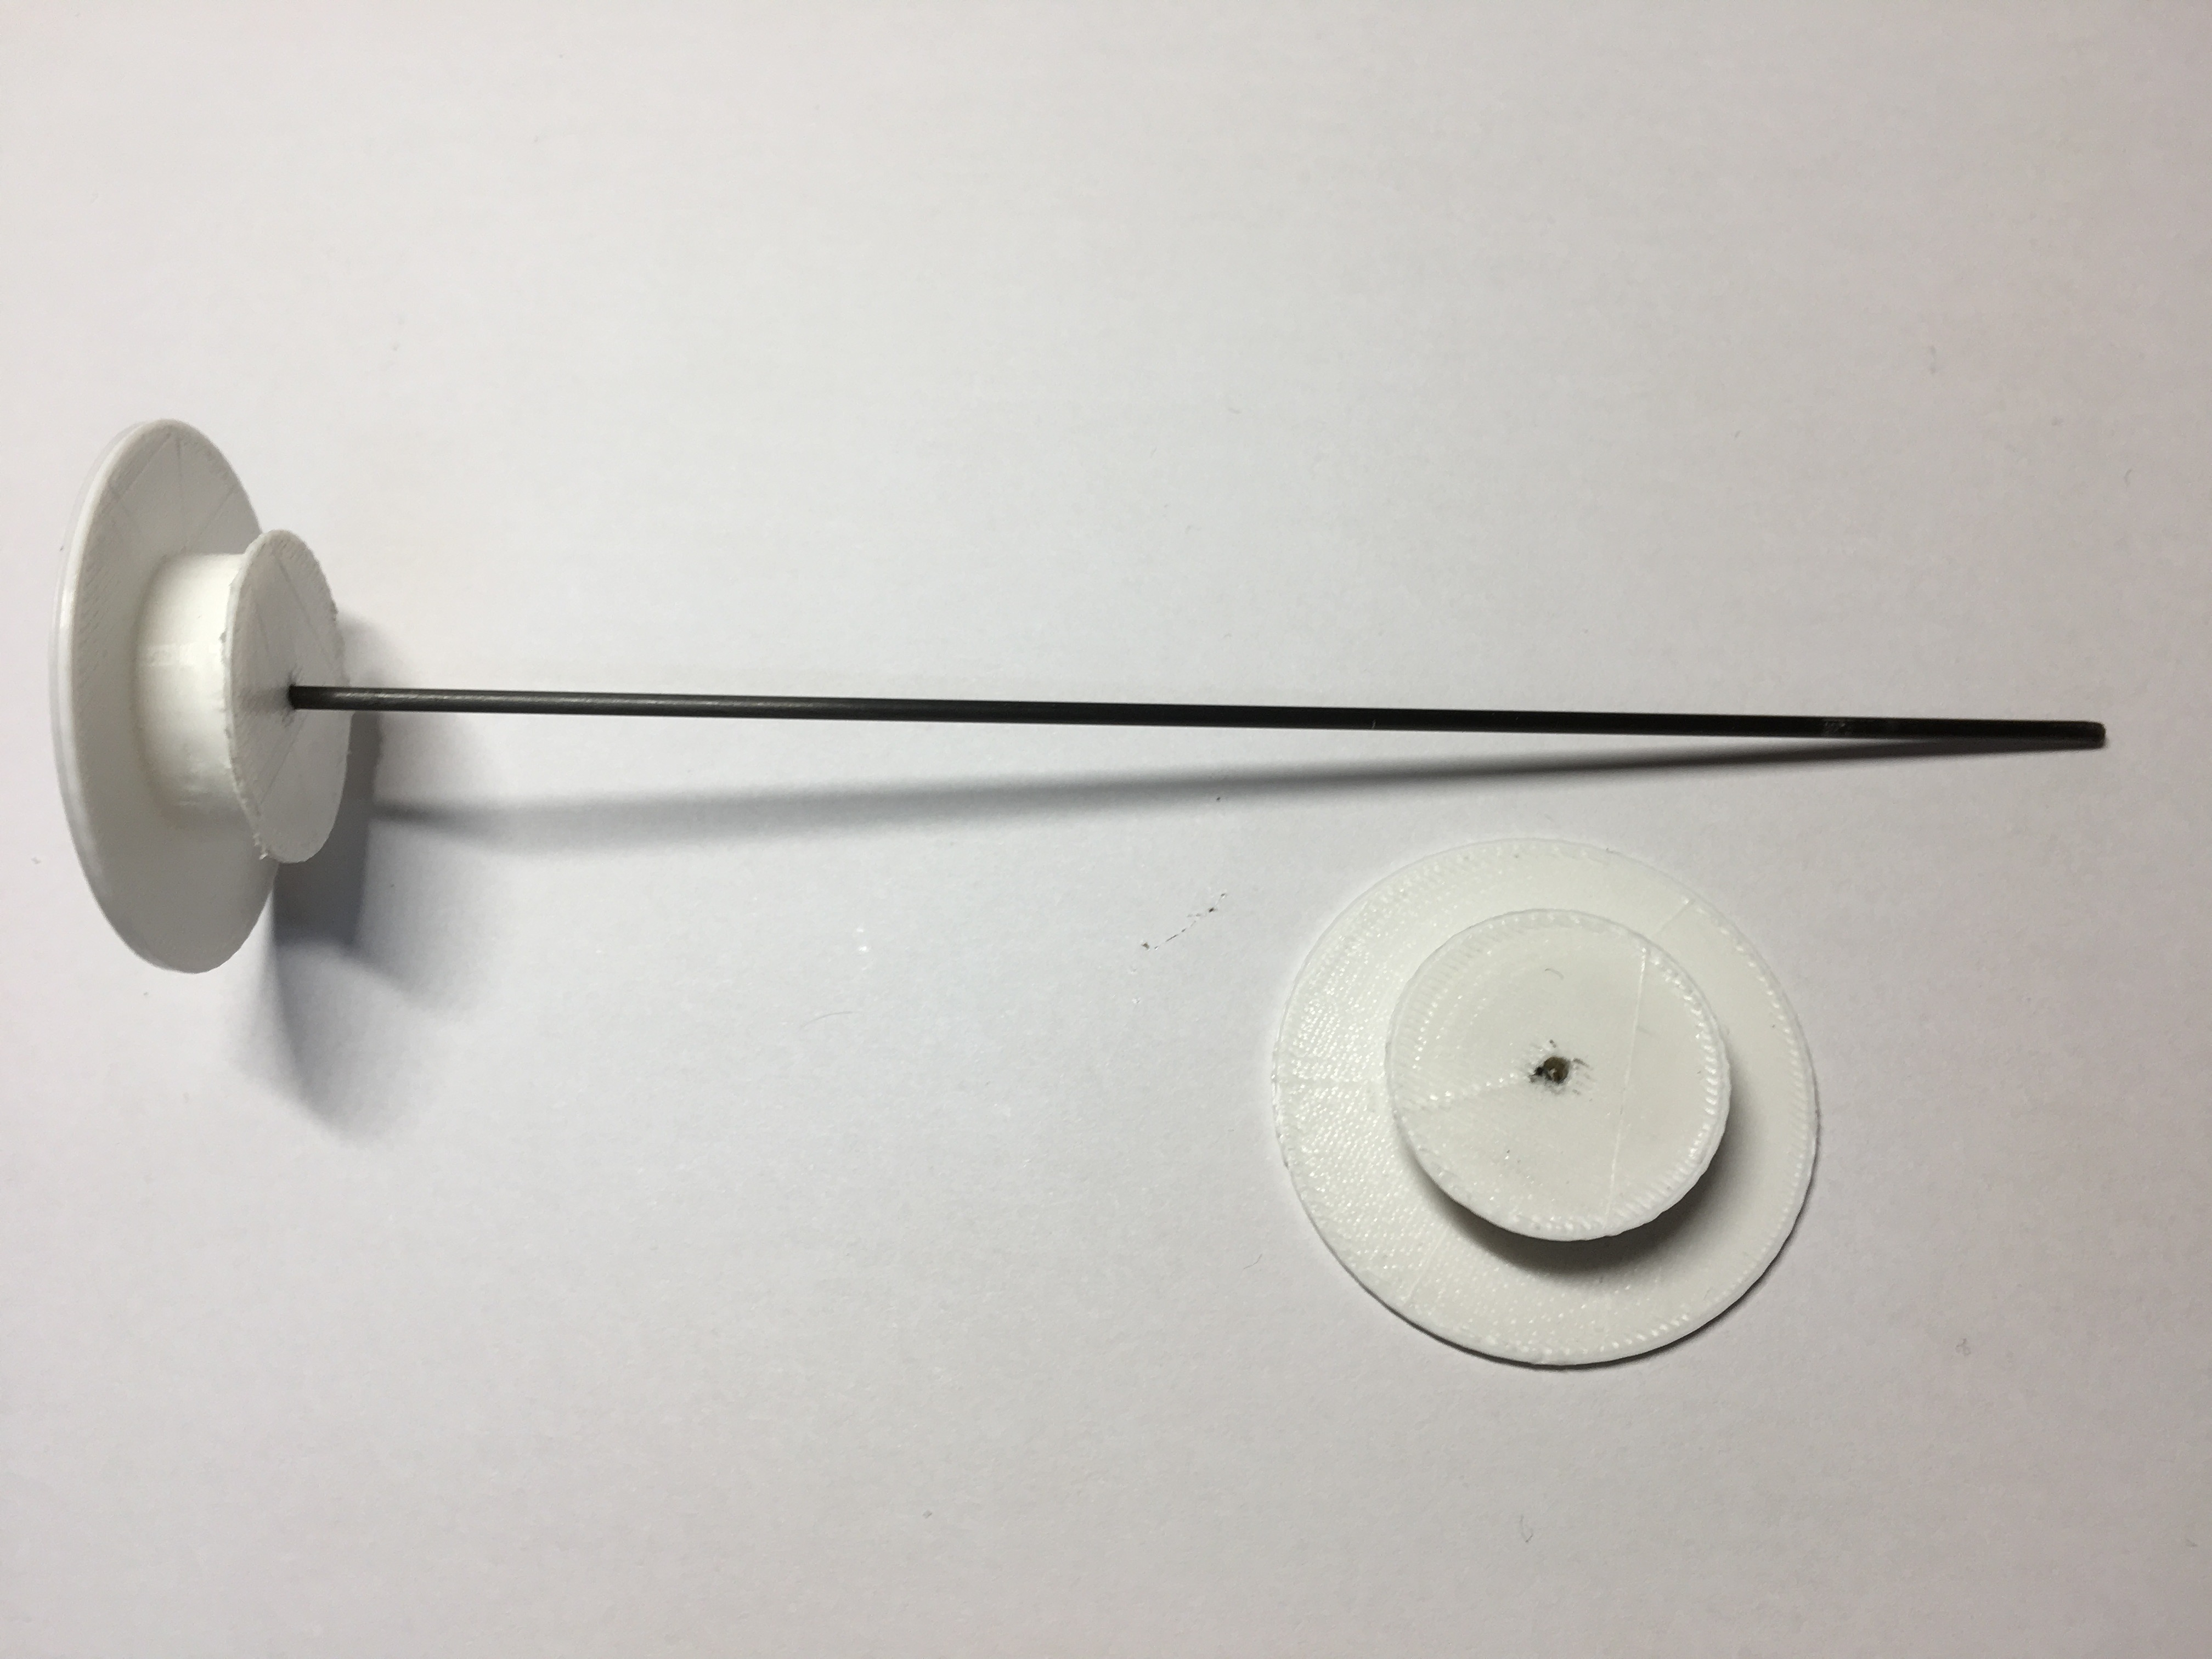
\includegraphics[height=10cm]{figure/procedure/p5}
 	\caption{Two wheels on the axle. \label{fig:twoWheels}}
	\end{figure}
	\item Insert two wheels onto the axle.
	\item Stick a servo at the base using 3M tape with a steering wheel fixed on it.
	\item Stick a voltage transformer at the back of the base using 3M tape. Caution: Use multiple layers of tape to make sure the transformer strongly sticked to the board.
	\item Stick a battery on the base using 3M tape. \\
	\begin{figure}[H]
	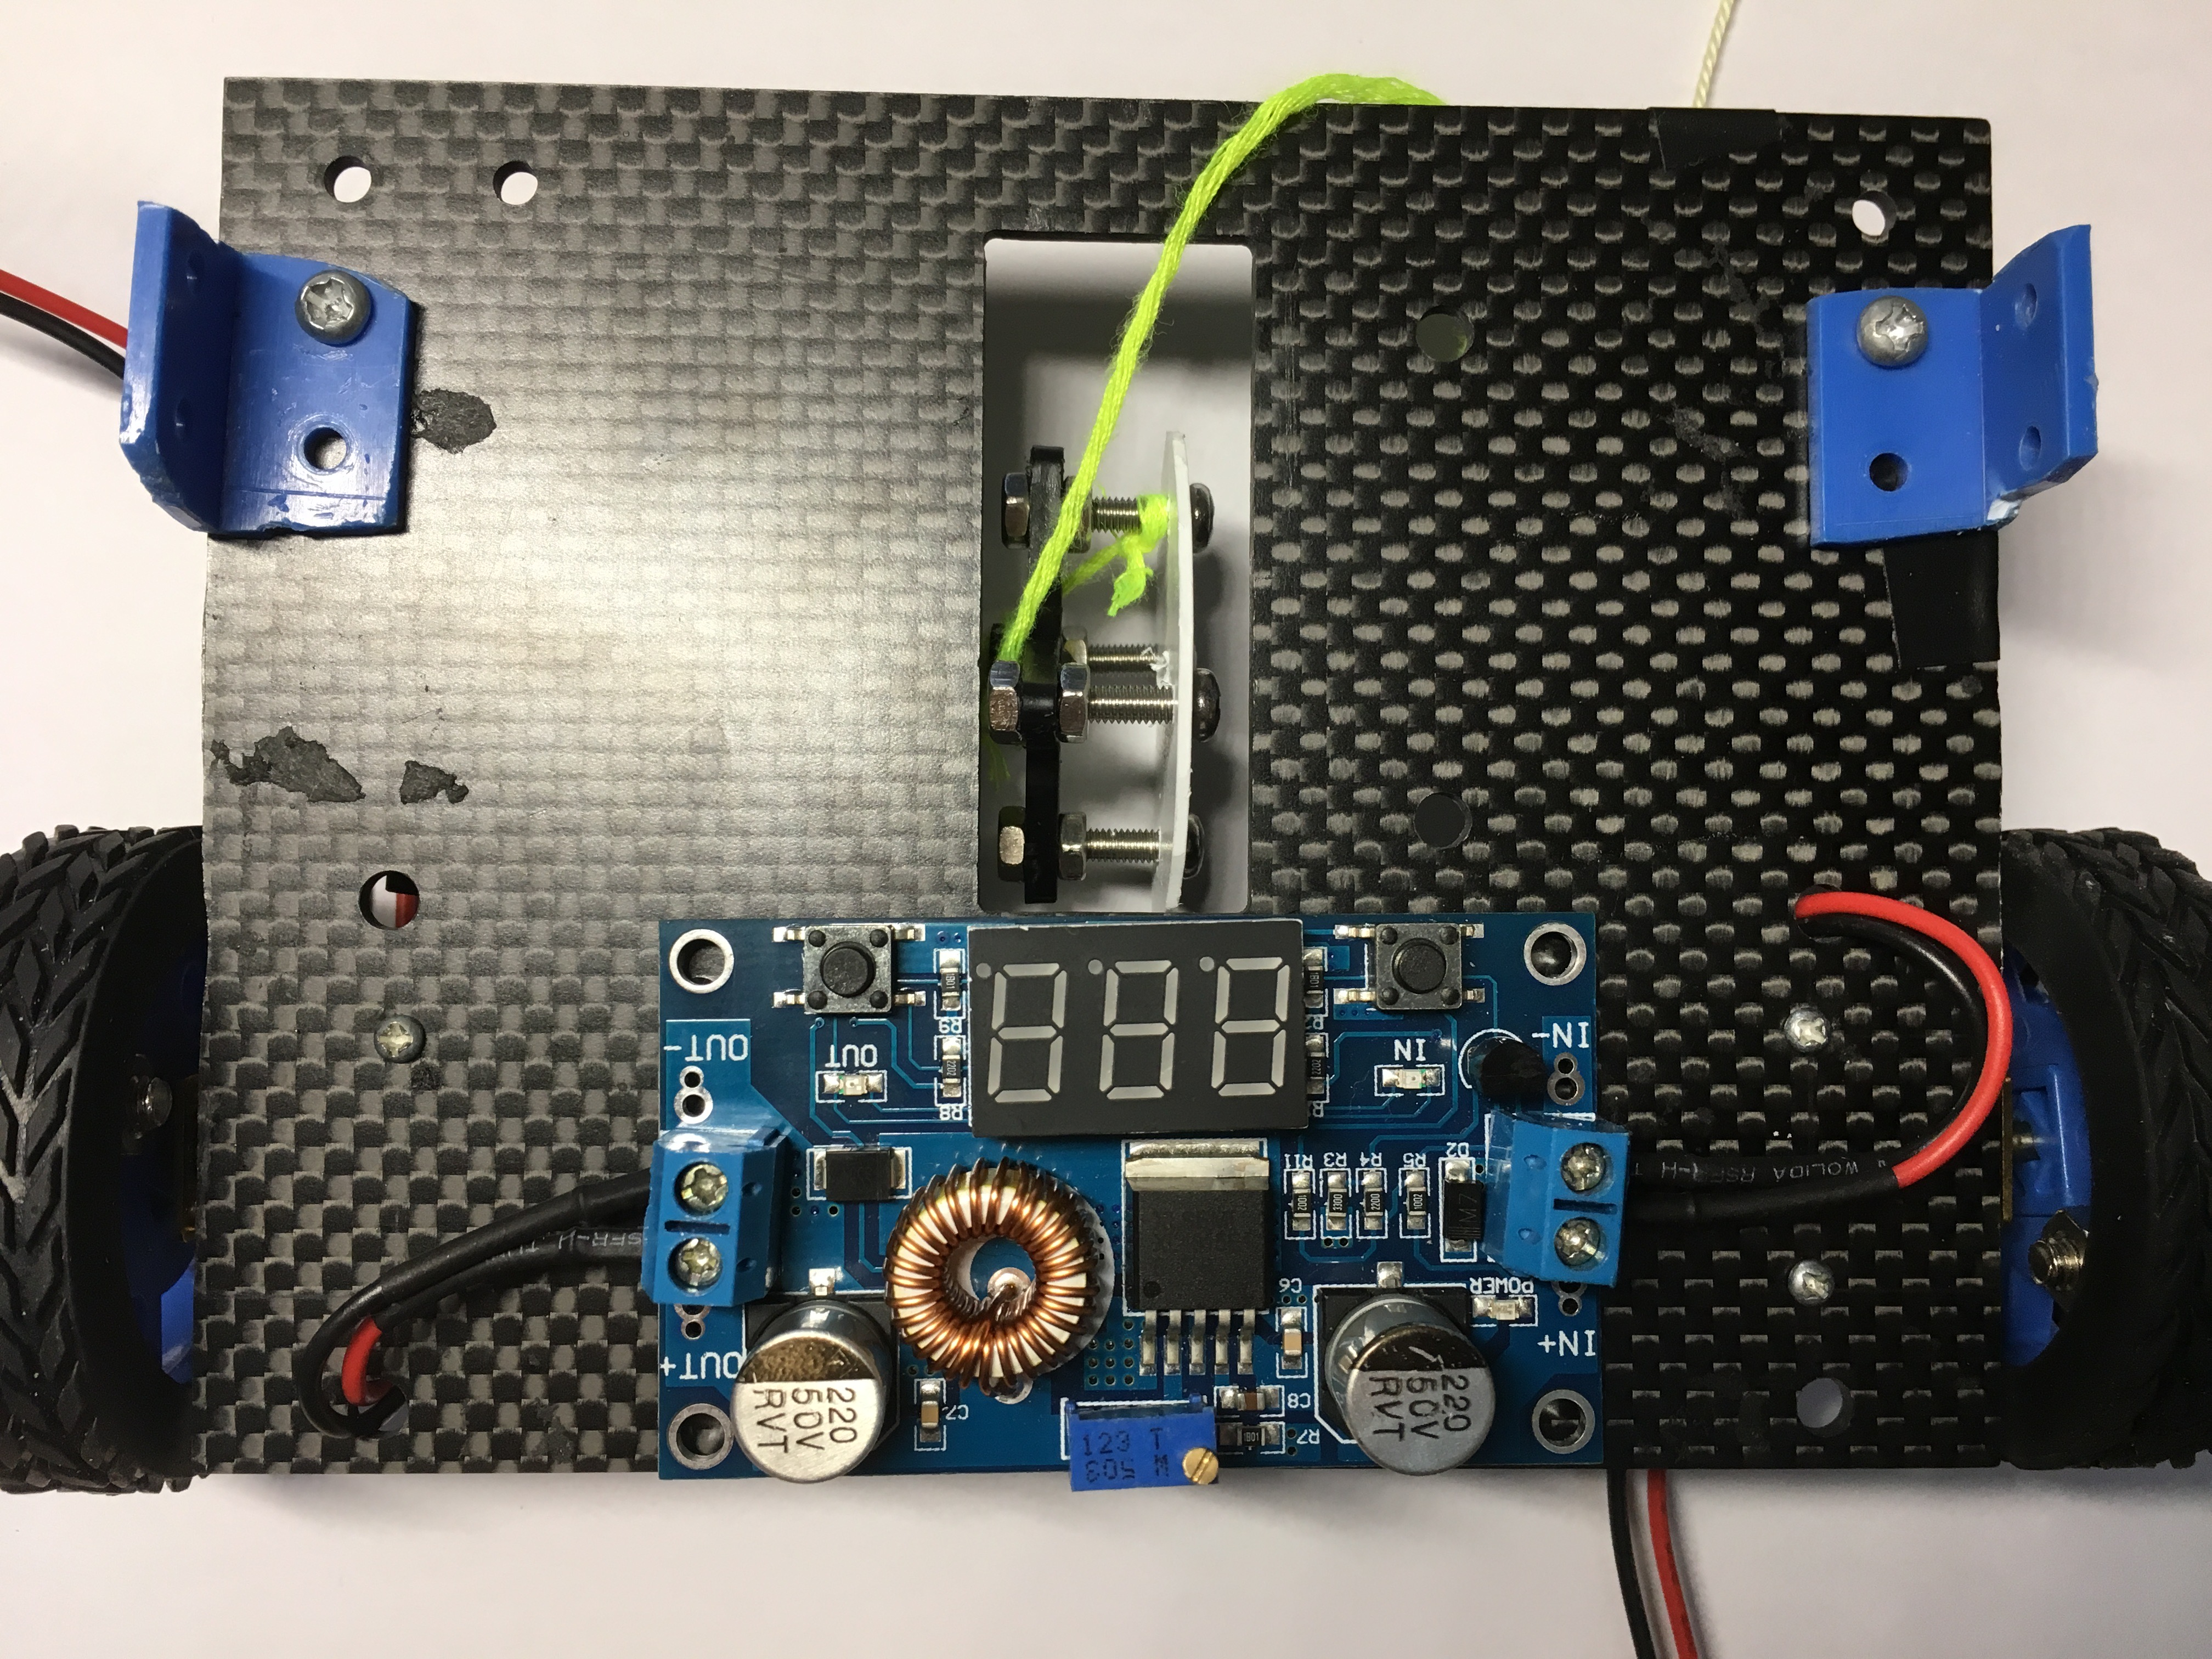
\includegraphics[height=10cm]{figure/procedure/p6}
 	\caption{Assembling the motor driver. \label{fig:assMotor}}
	\end{figure}
	\item Assembling the motor driver with two motor using tin solder. Caution: tin solder is very dangerous. Do not let your skin contact with tin when it is still hot.\\
	\begin{figure}[H]
	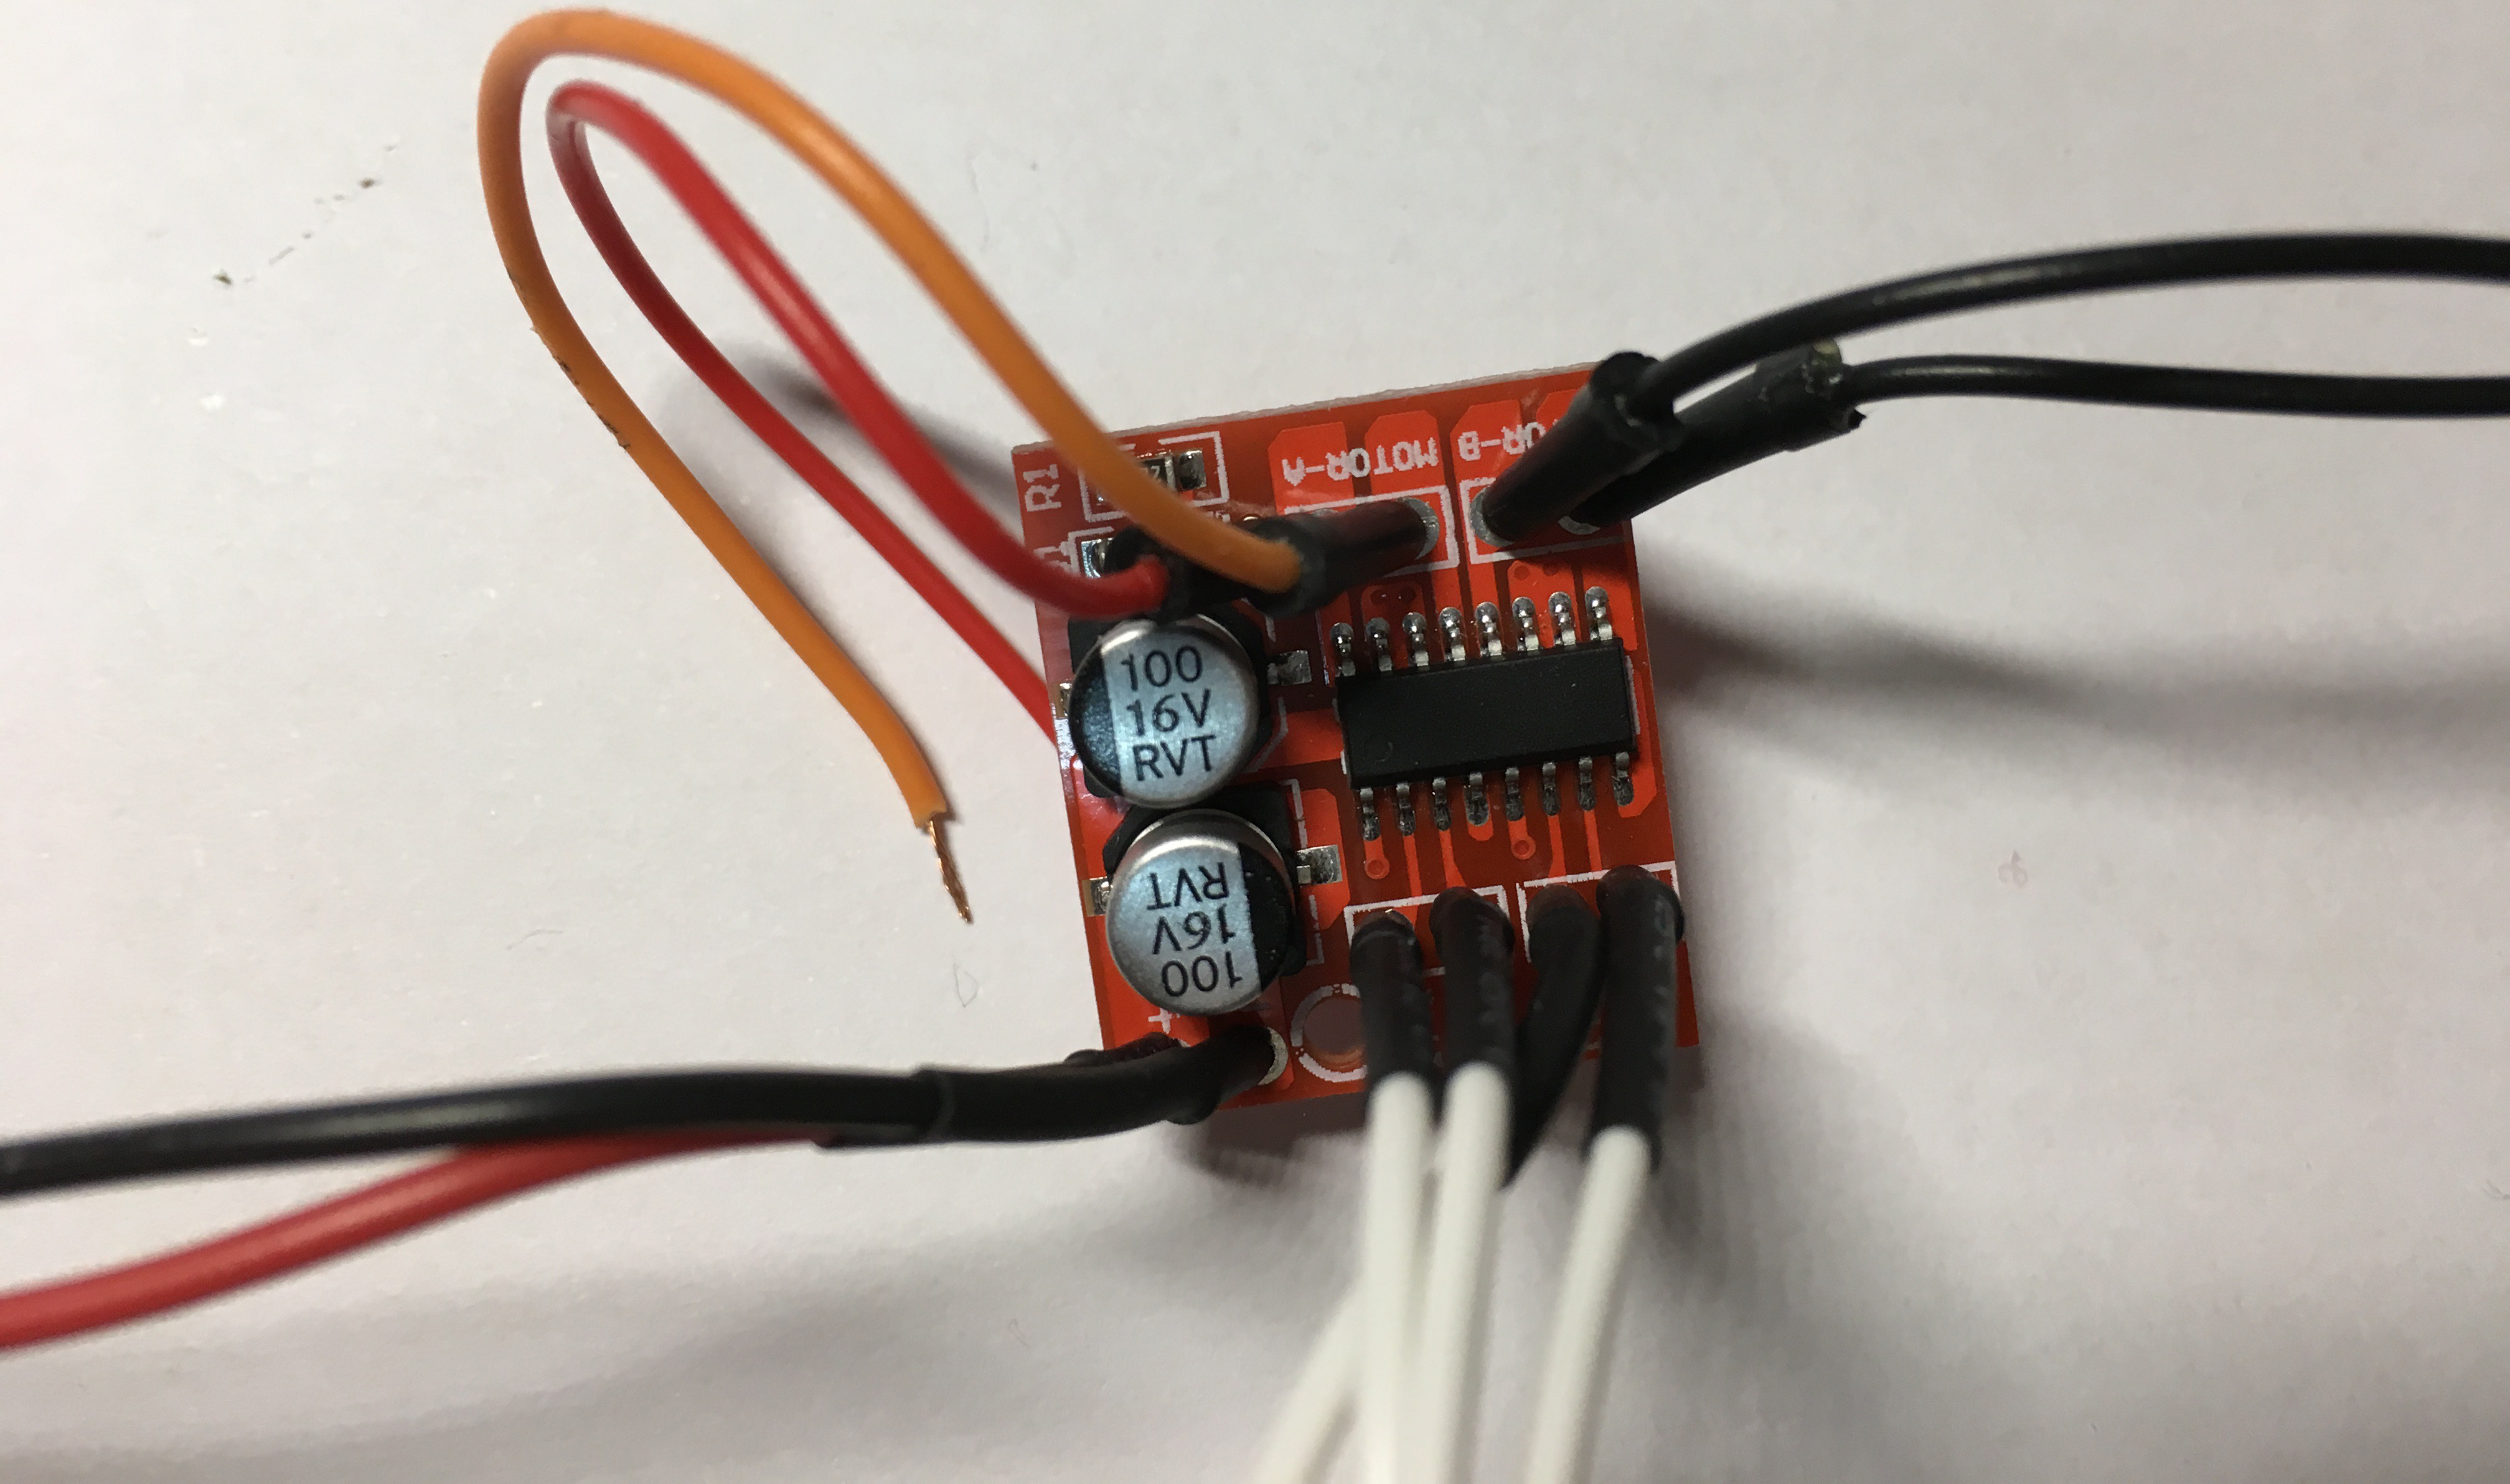
\includegraphics[height=10cm]{figure/procedure/p7}
 	\caption{Arduino UNO board. \label{fig:ardUnoBoard}}
	\end{figure}
	\item Stick the Arduino UNO board on to the battery using 3M tape.
	\item Finish the assembling according to the circuit diagram. 
	\item Put wires in order and bind them together using Electrical tape. 
	\end{enumerate}
\item Design the rope
	\begin{enumerate}
	\item Make a knot that can adjust the length of the rope.
	\item Bind the rope to the hook. 
	\item Fix them with 502 glue.
	\end{enumerate}
\end{enumerate}
